Finally, we can briefly discuss the diagrammatic representations of the CC approximations up to and including the triples approximation. In this chapter, we will only mention some of the crucial diagrams. For a complete derivation of the coupled cluster diagrams up to and beyond the triples level, see, for example, Ref. \cite{Ref21}.

To the diagrammatic rules we developed in Chapter 2 of this thesis, we can also add the following diagrammatic rules, which are specific to drawing coupled cluster diagrams:

\begin{itemize}
    \item Every vertex representing $\hat{T}_m$ picks up a factor of $\langle a_1 ... a_m | \hat{t} | i_1 ... i_m \rangle$ (the T-amplitudes)
    \item Each pair of $\hat{T}_m$ vertices which are equivalent pick up a factor of 1/2.  The vertices are equivalent if they connect to the interaction vertex in the same way.
\end{itemize}

Representing the $\hat{T}_1$, $\hat{T}_2$, and $\hat{T}_3$ operators in diagrammatic representation is quite simple, and these are shown in Fig. \ref{fig:T_diagrams}.

\begin{figure}
    \centering
    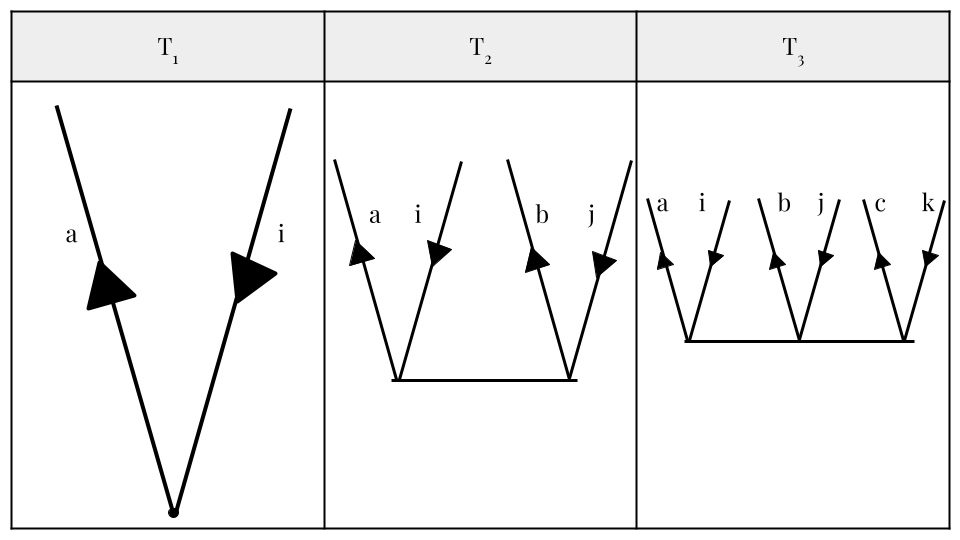
\includegraphics[scale=0.25]{Images/Chapter3/CC_diagrams.png}
    \caption{Diagrammatic representations for the $\hat{T}_1$, $\hat{T}_2$, and $\hat{T}_3$ operators.  Higher order $\hat{T}_m$ operators can be created using the pattern in the operators shown here.}
    \label{fig:T_diagrams}
\end{figure}

To show a complete coupled cluster calculation written out in diagrammatic form, we will represent the CCD amplitude equation in diagrammatic form in Eq. \ref{fig:ccd_amp}.  Though long, this collection of diagrams is significantly shorter than the entirely written out CCD amplitude equation using summations and Dirac notation, which can be found in Ref. \cite{Ref8}.

\begin{figure}
    \centering
    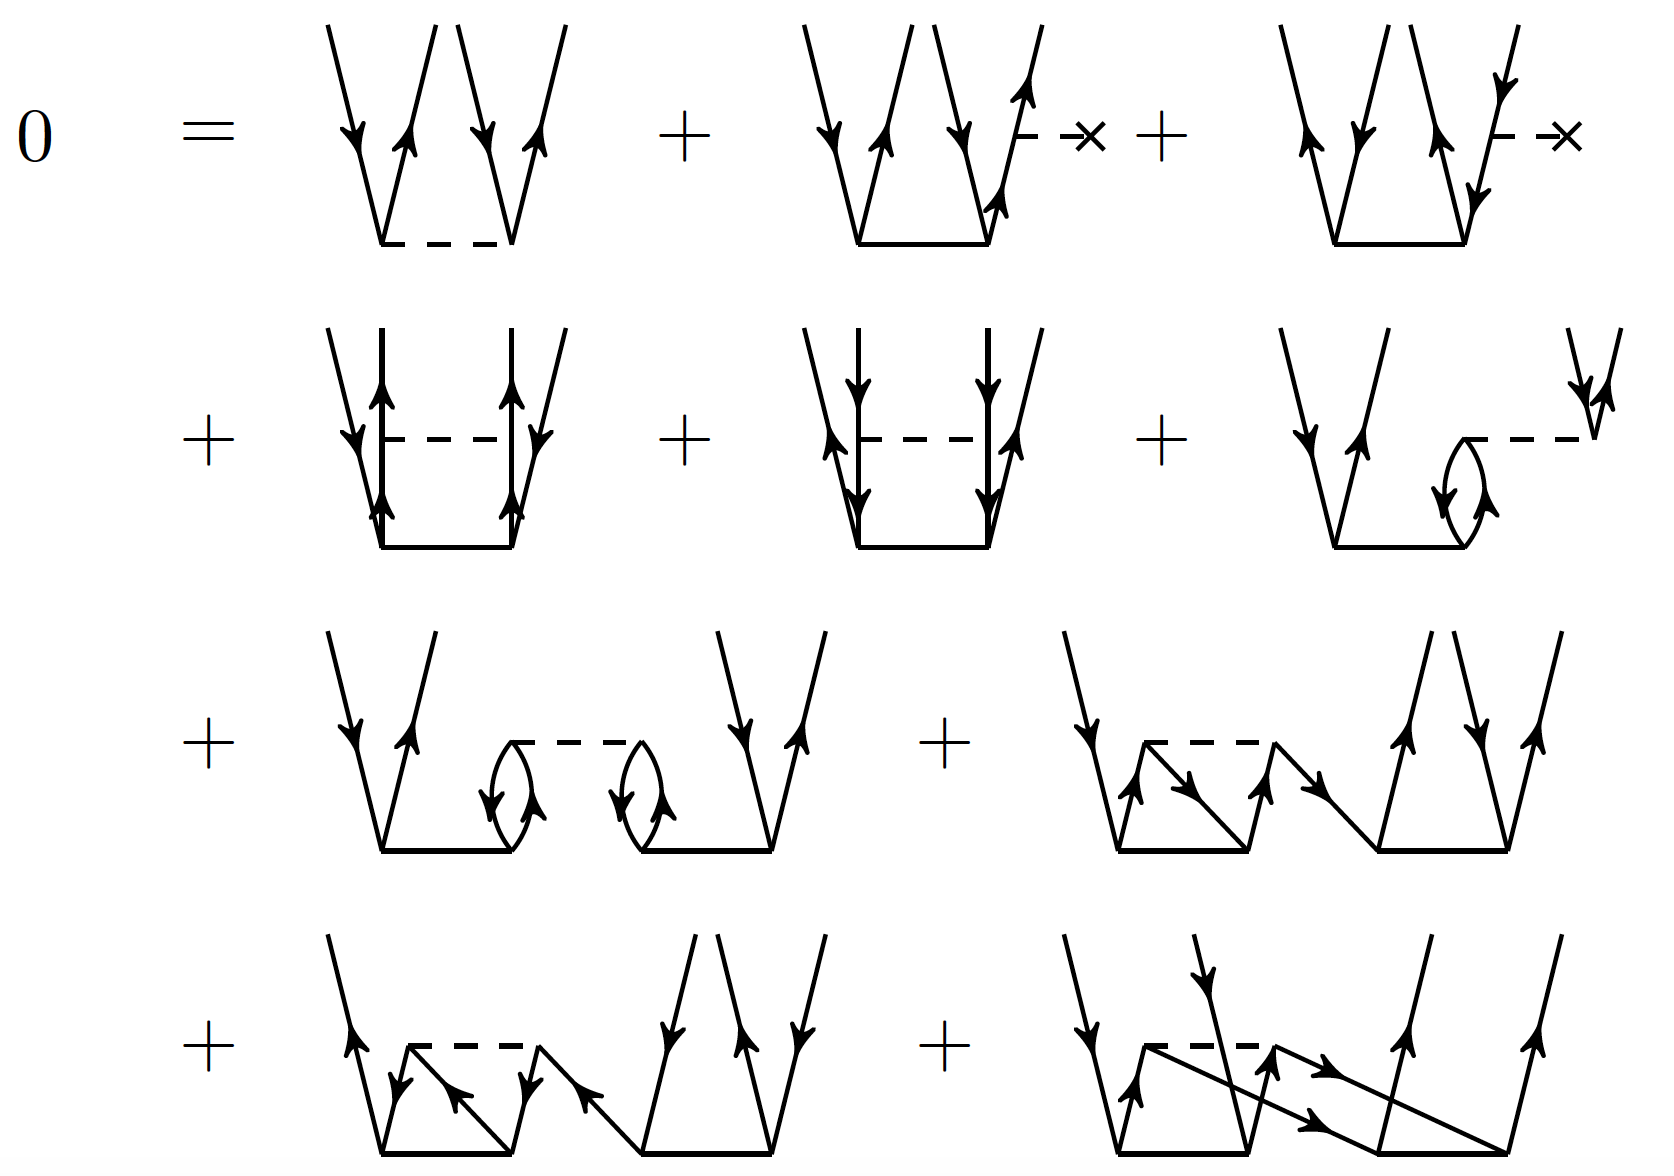
\includegraphics[scale=0.25]{Images/Chapter3/Diagrams-CCD.png}
    \caption{The diagrammatic formulation for the CCD amplitude equation.}
    \label{fig:ccd_amp}
\end{figure}



\begin{figure}
    \centering
    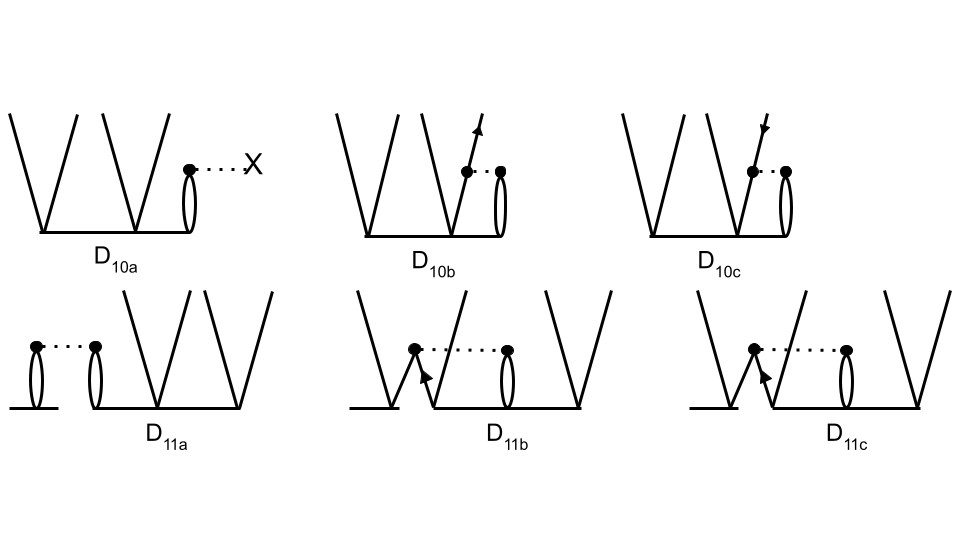
\includegraphics[scale=0.25]{Images/Chapter3/T3 to CCSDT T2.png}
    \caption{Antisymmetrized Goldstone diagrams representing the $\hat{T}_3$ contributions to the CCSDT $\hat{T}_2$ equations. D$_{10b}$ and D$_{10c}$ are relevant to the CCDT-1 approximation defined in the last section.}
    \label{fig:my_label}
\end{figure}

\begin{figure}
    \centering
    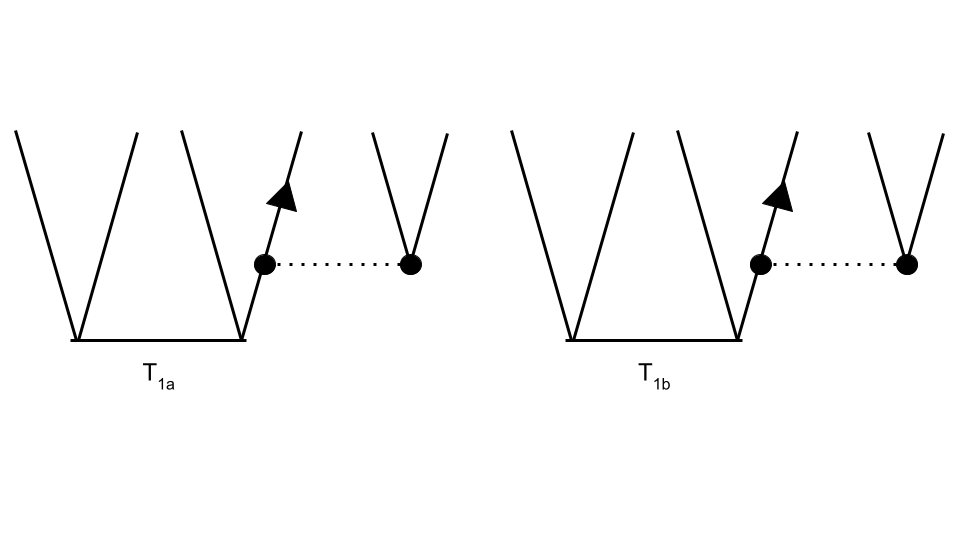
\includegraphics[scale=0.25]{Images/Chapter3/Relevant T3.png}
    \caption{Antisymmetrized Goldstone diagrams representing the CCSDT $\hat{T}_3$ equations relevant to calculating the CCDT-1 approximation. For a full list of all antisymmetrized Goldstone diagrams for the CCSDT $\hat{T}_3$ equations, the reader is referred to Ref. \cite{Ref21}.}
    \label{fig:my_label}
\end{figure}

Finally, look at some diagrams from the $\hat{T}_3$ operator, which are important to the CCD(T) and CCDT-1 approximations. In fact, the terms $T_{1a}$ and $T_{1b}$ from the $\hat{T}_3$ amplitude equations form  Eq. \ref{ccdt1_eq}.  The amplitudes that are gained by this equation are then used to calculate the diagrams $D_{10b}$ and $D_{10c}$ for the $\hat{T}_2$ amplitudes \cite{Ref156}.